\chapter{Related Work}

\begin{flushright}{\slshape
The old computing was about what computers could do; the new computing \\
is about what users can do. Successful technologies are those that are\\
in harmony with users' needs. They must support relationships and \\
activities that enrich the users' experiences. } \\ \medskip
	    --- Ben Shneiderman
	\end{flushright}

In this chapter we describe related work. The work can be related in several ways, depending on which aspect of the work is considered. Therefore the chapter is subdivided into five sections, each devoted to one aspect. These are Related projects and frameworks (Section \ref{RelatedProjects}), Ubicomp ontologies (Section \ref{UbicompOntologies}), Interaction models (Section \ref{InteractionModels}), Task models (Sections \ref{interactionTasks}) and Semantic models (Section \ref{interactionFrogger}).






\section{Related projects and frameworks}
\label{RelatedProjects}
% Possible TODO Amigo, Embassi
% 
% \subsection{Amigo}
% 
% The Amigo project\footnote{http://www.hitech-projects.com/euprojects/amigo/} is a European project that ran from 2005 to 2008. 

In the field of ubiquitous computing there are a substantial number of past and current projects and relevant software frameworks that exist, most of them in the area of context-aware computing. In the following sections we will focus on those projects that are the closest in scope to the issues that are addressed by the work described in this thesis:

\begin{itemize}
	\item Serendipitous interoperability, as addressed by the \emph{recombinant computing} approach of the SpeakEasy project
	\item Sharing information between devices, as addressed by the Event\-Heap shared event system and its tuple space protocol
	\item Using one device to control another, as addressed by the \emph{opportunistic assemblies} of the the XWeb architecture
	\item Multi-device user interaction, as addressed by the \emph{Media Cubes} of the AutoHAN project
	\item Configuring connections between devices, as addressed by the \emph{plug-synapse model} of the e-Gadgets project
\end{itemize}



\subsection{SpeakEasy}

We cannot expect all devices to have a priori knowledge of all the other devices they might possibly be connected to. We can, however, expect users to have knowledge about the devices they might encounter in their environment. Even if my smart phone does not know how to communicate with a specific printer, the software infrastructure could provide the necessary technical building blocks to allow them to communicate. The user understands what a printer does and makes the decision to connect the smart phone to the printer, as well as what to print.

% Begin TiiS
% (this is in introduction)
% According to Newman et al. \cite{Newman2002}, the following should be communicated to the user:
% \begin{itemize}
% \item What devices and services are available
% \item Capabilities of the devices and services
% \item Relationships between each another and the environment
% \item Predictions of likely outcomes from interaction
% \end{itemize}

This line of thinking was a starting point for Newman et al \cite{Newman2002}, who developed an approach which they named \emph{recombinant computing}, used in the SpeakEasy project at Xerox PARC. With this approach components are designed with the thought that they may be used in multiple ways, under different circumstances and for different purposes. Components expose \emph{recombinant interfaces} that are simple, domain-independent programmatic interfaces governing how components can interoperate with one another.
% End TiiS

\label{InformationFiltering} % this part on information filtering was on Notational Velocity
The SpeakEasy project focused on what users might be trying to accomplish in a specific situation when connecting entities to one another. Possible examples include connecting devices in order to give a presentation, or in order to send contact information. They created templates of common tasks that contained a partially specified set of connections and entities, which could be fully specified and instantiated by users at run-time. An instantiated template was then added to a list of current tasks. It was noted that templates impose a layer of semantics on top of the raw infrastructure. Templates assisted users by constraining the available component choices to only those that were appropriate for the task at hand.

The SpeakEasy environment consisted of a web application that allows users to browse for components, which can be viewed and organised in different ways, for example grouped by location or owner.\marginpar{The e-Gadgets project in Section \ref{egadgets} also made use of a web application to configure components.}

What can be learned from the SpeakEasy project is the importance of describing the interfaces of components, such that they can be combined with other components. These interface descriptions help to enable serendipitous interoperability, and described in more detail in Chapter \ref{DeviceCapabilityModelling}. 


\subsection{EventHeap}

Stanford University's shared event system, called the EventHeap, provides a base set of capabilities that link devices in a room \cite{Winograd2005}. It allows users to move data and applications between areas, for example redirecting a pointer from one device to another. One of these devices, the DynaWall, is a wall-size touch-sensitive interactive display. Gesture-based interaction facilitates moving information objects from the wall from one side to another, by throwing and shuffling visual objects with different accelerations and sounds.

During the development of their system, they identified the following design guidelines:

\begin{itemize}
	\item Heterogeneity - Devices must be able to interoperate in spite of heterogeneity in software. Interfaces must be customised to work smoothly on different-sized displays with different input/output modalities.
	\item Dynamism - A software framework must handle applications and devices joining and leaving, while minimising the impact on other entities in the space.
	\item Robustness - Users will treat the devices in interactive workspaces as appliances that should not fail in inexplainable ways. Devices must provide for quick recovery.
	\item Interaction techniques - A long, large wall needs an interaction technique suited to its size and location (such as DynaWall's throwing and shuffling technique).\marginpar{We explored similar interaction techniques during the development of the Spotlight Navigation device, see Section \ref{SpotlightNavigation} and \cite{Rapp2010}.}
\end{itemize}

Devices in EventHeap use a tuple space protocol to communicate with one another, where particular tuples have meaning to certain parties \cite{Edwards2001}. This semantic agreement between parties is implemented by the developer, for example a tuple representing a request to scan an image.

The iStuff toolkit \cite{Ballagas2003} was developed within Stanford to explore post-\ac{GUI} interaction techniques, and makes use of the EventHeap system. The iStuff toolkit allows users to map wireless input devices like buttons, sliders, wands, speakers and microphones to different applications running on devices like the DynaWall.

% from TiiS paper

Patch Panel \cite{Ballagas2004} is a mechanism in the iStuff toolkit that tries to solve incremental integration, the problem of integrating new devices and applications that may not have a priori knowledge of each others existence of function. They noted that SpeakEasy allows for direct user intervention via \acp{GUI}, but does not support automated connections free of user intervention, for example data from presence sensors that may be used to turn on the lights. Patch Panel uses an approach called intermediation, with a decoupled communication model (such as publish/subscribe) for inter-component communication. \marginpar{A similar decoupled model was used for the work described in this thesis.} Patch Panel uses a set of mappings between triggers and output events to enable intermediation. These mappings are defined using the Patch Panel Manager \ac{GUI} or \ac{FSM}-based scripting language, and users configure connections using a web-based configuration wizard.

% end TiiS


\subsection{The XWeb architecture}
The goal of the XWeb architecture \cite{Olsen2001} is to allow for \emph{opportunistic assemblies} of interactive resources in order to accomplish a particular task. Olsen et al recognised that both an interactive model for acquiring and using the interaction resources, as well as an underlying infrastructure is needed. In their model, each interaction resource resolves user intent independently, instead of merging inputs from a variety of modalities.

A client-server architecture was used to create the infrastructure, with \ac{XML} objects used to model resources and services. Tasks were defined using a two-part \ac{URL} in the form \texttt{dataReference::viewReference}, where the \emph{view} is an abstract definition of a particular interaction. These views are defined as a tree of \emph{interactors}, where the data and the view of the current task as well as the path of the interactor is used to characterise the current state of the device.

XWeb uses a subscribe mechanism to allow multiple clients to share their information, where the devices themselves are not aware of each other but can still be integrated into the same task. The problem that is addressed is that the different devices can be connected without requiring a lot of configuration effort from the user.

Pierce and Mahaney \cite{Pierce2003} extended the XWeb approach to opportunistic assemblies with \emph{opportunistic annexing}, which is is the process of temporarily attaching one or more resources, like a speaker or a keyboard, to a device in order to enhance its capabilities. Opportunistic annexing differs from the other approaches in this section in that it extends the existing capabilities of devices, instead of assembling heterogeneous devices into a larger, aggregate device. A higher-level description of user's actions, instead of raw input events, reduces the communication load and the amount of raw input events that need to be understood by the device itself. 


\begin{table}
    \myfloatalign
  \begin{tabularx}{\textwidth}{Xll} 
	\toprule
    \tableheadline{Name} & \tableheadline{Scale} & \tableheadline{Examples} \\ 
    \midrule
	Covert & 1 cm & Watch, RFID badge, Bluetooth headset \\ %, iPod Shuffle
	Mobile	& 10 cm	& Laptop, camera, mobile phone \\ % e-book reader, 
	Personal & 1 m & ATM, desktop computer, automobile \\ %Microsoft Kinect, 
	Environmental &	10 m &	Television, Public display, Nintendo Wii \\
	Architectural & 100 m & Media facade, Arena scoreboard\\ %, Interactive art installation \\
	Urban & 1 km & Temporary giant ubicomp experiences \\
	
    \bottomrule
  \end{tabularx}
  \caption{Kuniavsky's Scales of Ubicomp Device Design}
  \label{MultiScale}
\end{table}

Opportunistic annexing allows interaction at one scale to be controlled by a device at a different scale. Kuniavsky \cite{Kuniavsky} defined the scales of ubicomp device design shown in Table \ref{MultiScale}. The name of each scale is meant to convey the size of devices at that scale, similar to Greenfield's \cite{Greenfield2006} description of \emph{everyware}, acting ``... at the scale of the body, [...] the room, [...] the building, [...] the street, and of public space in general''.

Pierce and Mahaney expect that the primary benefit of annexing input resources will be faster input rates. This means that the actual annexing action should be faster than the time required to perform the action. For example, if a user will save 5 seconds by typing a note on a keyboard rather than on a mobile device, annexing the keyboard to the mobile device should take less than 5 seconds.

\subsection{AutoHAN}

AutoHAN is a networking and software architecture to enable user-programmable specification of interaction between appliances in a home environment \cite{Blackwell2001}. It tries to solve the issue of potential complexity between digital devices that interact with each other, especially if these devices are manufactured by different companies (as it is the user who has to specify how they will interact with one another).

%Blackwell considers direct manipulation to be far more important than pictorial metaphors for assisting end-users in learning a novel programming language. 
Blackwell distinguishes between two different abstractions that users have to consider:
\begin{itemize}
	\item \emph{Abstraction over time}, where an appliance has to do something in the future, for example recording a TV programme
	\item \emph{Abstraction over a class} of entities, where the user is referring to a set of entities, for example a playlist of music
\end{itemize}

\marginpar{The representations of AutoHAN's abstractions are notational systems, validated by the Cognitive Dimensions framework discussed in more detail in Section \ref{CognitiveDimensions}.}

Within the AutoHAN project the \emph{Media Cubes} language was created --- a tangible representation of an abstract situation. Each cube has a button for input, and a LED and piezo-electric transducer for feedback. Cubes communicate with the AutoHAN network via infrared ports, and use induction coils on four faces of the cube to detect proximity to other cubes. By holding one face of a cube against an appliance, the cube can be \emph{associated} with some function of that appliance. Each individual cube is regarded by the user as a direct manipulation interface to some appliance function, where many different devices may implement this function. This is in contrast to a remote control, that is dedicated to a single appliance but provides access to many different functions.\marginpar{The cubes of the AutoHAN project can be viewed as a forerunner to the cubes used with our Interaction Tile (described in Section \ref{InteractionTile}), except that the AutoHAN cubes represent tasks, whereas the Interaction Tile cubes represent devices.} 

Each cube has a unique identifier, and each face of the cube can also be identified. This means that a combination of cubes and neighbouring faces can be used as a type of programming language. Cubes may also be associated with virtual devices: software components running somewhere on the network. The user regards these virtual devices to be the same as physical appliances that are placed in the broom cupboard, like a network router or home server.

AutoHAN devices communicate using \ac{UPnP} \ac{GENA}. \ac{GENA} is a publish/subscribe system that uses HTTP as transport mechanism. It defines three new HTTP methods to manage event subscriptions and deliver messages:

\begin{itemize}
	\item SUBSCRIBE to subscribe to event notifications and renew existing subscriptions
	\item UNSUBSCRIBE to cancel a subscription
	\item NOTIFY to send an event notification to a subscriber
\end{itemize}

AutoHAN entities make subscription requests to receive certain types of events. When such an event occurs, an HTTP NOTIFY request is sent to the subscriber, with additional parameters (such as which button on a control panel was pressed) are encoded in the \ac{GENA} Notification subtype or in the message body.

Two alternative programming paradigms were considered for the Media Cubes language - an \emph{ontological paradigm} and a \emph{linguistic paradigm}. In the ontological paradigm, tokens represent ``natural categories'' in the user's mental model. Concepts were identified which have a close correspondence between primitive remote control operations, appliance functions, capabilities and user skills, representing a primitive ontology of home automation. These abstract types were incorporated into four cubes:

\begin{itemize}
	\item The \emph{Event} cube (``on''/``off'', ``go''/``stop'') represents a change of state, such as a sensor activation (e.g. a doorbell) or automated function (e.g. alarm clock). ``Go'' and ``on'' is functionally identical, but labeled separately to help users reason about equivalence between events and processes.
	\item The \emph{Channel} cube can be used to associate a media channel/stream with a media source, and direct the stream to a media sink.
	\item The \emph{Index} cube selects content from a channel and can be associated with particular index values, to select content that matches that value. 
	\item The \emph{Aggregate} cube allows the user to refer to abstract collections rather than individual instances.
\end{itemize}

In the linguistic paradigm, cubes represent words in a language, for example a single face of a cube may be labelled \emph{Clone}. When this face is placed against another cube face and activated, the second face takes on the identity and function of the first. A \emph{List} cube has three active faces: Add Item, Remove Item and Contents.


\subsection{e-Gadgets}
\label{egadgets}

The e-Gadgets\footnote{http://extrovert-gadgets.net/} project was a European project within the Disappearing Computer initiative. An architectural style, called \ac{GAS}, was developed for devices to communicate with one another. To evaluate \ac{GAS}, a supporting infrastructure and computationally enhanced artefacts, called e-Gadgets, were created.

Mavromatti et al. \cite{Mavrommati2004} developed an approach to allow users to treat these e-Gadgets as reusable components which can be connected to one another. They defined the following requirements for such a system:

\begin{itemize}
	\item Devices should interoperate via a universal system architecture that accommodates existing communication protocols, e.g. WiFi and Bluetooth.
	\item Tools and interfaces should allow people to control devices and services. These can either be contained within existing devices or created for a specific purpose.
	\item Invisible connections will exist between the different physical and virtual devices. Tools must visualise this device structure, make device states visible, explain device functionality and help people to manage the inter-device associations.
\end{itemize}

The \ac{GAS} defines a set of concepts and rules in an ontology, a middleware, a methodology and a set of tools that enable people to compose distributed applications using services and devices in an ubiquitous computing environment. At the conceptual level, \ac{GAS} specifies a \emph{plug-synapse} model, where device capabilities are visualised in the form of \emph{plugs}. Plugs can be associated with one another, creating \emph{synapses} between devices.

Plug descriptions are defined in \ac{XML}, using a DAML+OIL ontology, and linked to a unique device identifier. DAML+OIL, a combination of the \ac{DAML} and \ac{OIL} markup languages, has been superseded by \ac{OWL}. 

Synapses and plugs are viewed and modified using an \ac{GUI} editor. A concept evaluation was performed with the editor to test the comprehensibility of the concepts and the willingness to use such a technology. The Cognitive Dimensions framework was used to perform the evaluation. This framework was also used for evaluations of the work described in this thesis, and is discussed in more detail in Section \ref{CognitiveDimensions}. Results from the evaluations include the following:

\begin{itemize}
	\item Users will use their experience gained through a trial-and-error process to bridge the gap between their intentions and the feedback gathered through their actions.
	\item A device can be part of multiple in-home applications at the same time. The effect from interacting with that device is not clear based on physical appearance alone.
	\item A state change in one device could create a non-visible state change on another device.
\end{itemize}

They also noted that the possibility to combine the functionality of devices opens up possibilities for emergent behaviour, where the emergence results from how the devices are actually used. 

The rest of the chapter will introduce ontologies considered to be state-of-the-art  in ubiquitous computing, as well as related interaction models, task models and semantic models.

\section{Ubicomp ontologies}
\label{UbicompOntologies}
In this section we will look at the various ubicomp ontologies that have been developed for context-aware computing. The ontologies described later in this thesis builds upon this existing work, but with a stronger focus on interaction-related aspects. 
 
%We also hope to use the low-level events and command currently implemented in the system to automatically infer higher-level tasks and goals, with the final step being able to model the user's (and/or agent's) intentions using an ontology.

% start SISS2010
\subsection{SOUPA}

Chen et al. \cite{Chen2004} created \ac{SOUPA}, a context ontology based on \ac{OWL}, to support ubiquitous agents in their \ac{CoBrA}. The ontology supports describing devices on a very basic level (e.g. typical object properties are \texttt{bluetoothMAC} or \texttt{modelNumber}), but it has no explicit support for modelling more general device capabilities.

In the \ac{SOUPA} ontology, both computational entities and human users may be modelled as agents. An agent ontology is used to describe actors in a system, where actors include both human and software agents (or computing entities). In \ac{SOUPA} a computing entity is characterised by a set of mentalistic notions in the \ac{BDI} model, such as knowledge, belief, intention and obligation. The properties of a person agent includes basic profile information (name, gender, age etc.) and contact information (e-mail, phone number, mailing address etc.) \ac{SOUPA} references several domain ontologies to achieve this:

\begin{itemize}
\item \ac{FOAF}\footnote{http://http://www.foaf-project.org/} - one of the most well-known ontologies, used to describe people, their activities and relations to people and objects. \ac{SOUPA} uses \ac{FOAF} to express and reason about a person's contact profile and social connections with other people.
\item MoGATU BDI - an ontology developed by the same research group at the University of Maryland \cite{Yesha2004}, that describes an abstract semantic model for representing and computing over a user's or an agent's profile in terms of their prioritised and temporally ordered actions, beliefs, desires, intentions and goals. %\ac{SOUPA} uses this model to help independent agents to share a common understanding of their ``mental'' states, so that they can cooperate and collaborate. The agents also help to reason about the intentions, goals, and desires of the human users of a system. 
\end{itemize}

%start Some Reasoning Required
In a smart environment, we wish to infer a user's intention based on his/her context and interaction with the environment. In \ac{BDI} theory, a user's \emph{intention} is a \emph{desire} to which the user has committed. \emph{Goals} are desires which are consistent with one another. \emph{Plans} are a sequence of \emph{actions} to reach a specific goal. We can therefore infer intention based on an action, or sequence of actions. A sequence of actions (plan) to achieve a certain intention may be modelled using an ontology, and events are used to trigger the plan, update beliefs or modify goals.\marginpar{Modelling events is described in more detail in Chapter \ref{EventModelling}.}
%end Some Reasoning Required

The \ac{BDI} model is a philosophical model of human practical reasoning originally developed by Michael Bratman \cite{Bratman1987}, with a number of successful implementations and applications in the agent research community \cite{Bratman1988, Georgeff1996}. It could be argued that the \ac{BDI} model is somewhat dated, as the principles of the architecture were established in the mid-1980s and have remained essentially unchanged since then \cite{Georgeff1999}. 

A desire is the motivational state of an agent, with a goal having the added restriction that multiple active desires must be consistent (e.g. concurrent desires of ``going to a party'' and ``staying at home'' is not possible). When an agent commits to a specific plan with subgoals (based on a belief, or the informational state of the agent) it needs the capability to reconsider these at appropriate times when the world dynamics change. These committed plans and procedures are called intentions, or the deliberative state of the agent.

%When building intelligent pervasive computing systems, it may be useful to model computing entities as agents.

%end SISS2010

In an ontology, task models may be used to describe the user's actions, while the \ac{BDI} model may be used to represent the psychological, social and situational aspects of the tasks. Once the task model is defined, the system can adapt to the user, by mapping the user's current activity or task to higher-level goals and intentions. The \ac{BDI} model approach focuses on the anticipatory aspect of ambient intelligence, where the system tries to predict what the user is trying to accomplish.

When the goals, plans, desires, and beliefs of different agents are explicitly represented in the ontology, this information allows them to share a common understanding of their ``mental'' states, helping them to cooperate and collaborate. If we are able to represent the human user's mental states in the ontology, it may help software agents to reason about the specific needs of the users in a pervasive environment. 

\ac{SOUPA} covers contexts in the office/campus environment, but it has no explicit support for modelling general contexts in heterogeneous environments. 

\subsection{Gaia}
% Nixon and Ye worked on this
Ranganathan et al \cite{Ranganathan2004} developed an uncertainty model based on a predicate representation of contexts and associated confidence values. They incorporated this model into Gaia, a distributed middleware system for pervasive computing. Contexts are represented as predicates, following the convention that the predicate's name is the type of context being described (such as location, temperature, or time). This gives a simple, uniform representation for different kinds of contexts. Some contexts (such as \texttt{office}) are certain, whereas others (such as \texttt{location} and \texttt{activity}) might be uncertain. Uncertainty is modelled by attaching a confidence value between 0 and 1 to predicates. The context model is represented using \ac{DAML}+\ac{OIL}.

Ontologies are used in Gaia for the following:

\begin{itemize}
	\item Semantic discovery
	\item Matchmaking
	\item Interoperability between entities
	\item Interaction between human users and computers
	\item Context-awareness - physical, environmental, personal, social, application and system contexts are modelled
\end{itemize}

According to Ye et al \cite{Ye2007}, a set of lower independent profile ontologies should be built, each of which would reflect the characteristics of one aspect of a model of a person. These profile ontologies can then be customised and combined to satisfy particular application requirements.



\subsection{CAMUS}

Ngo et al. \cite{Ngo2004} developed the \ac{CAMUS} ontology in \ac{OWL} to support context awareness in ubiquitous environments. Their device ontology is based on the \ac{FIPA} device ontology specification\footnote{http://www.fipa.org/specs/fipa00091/SI00091E.html}, with every \texttt{Device} having the properties of \texttt{hasHWProfile}, \texttt{hasOwner}, \texttt{hasService} and \texttt{hasProductInfo}. Devices are further classified into \texttt{AudioDevice}, \texttt{MemoryDevice}, \texttt{DisplayDevice}, or \texttt{NetworkDevice}. For audio, the \texttt{hasParameter} property has the \texttt{Audio\-Parameter} class as range, with subclasses like \texttt{ACDC\-Parameter}, \texttt{In\-ten\-si\-ty} and \texttt{Harmonicity\-Ratio}. %Unfortunately it does not define a notion of completeness, and the ontology is thus not considered generic enough for general use in ubicomp environments.

One of the major goals of context-aware computing is to provide services that are appropriate for a person at a particular place, time, situation etc. In \ac{CAMUS}, context entities and contextual information are described in the ontology \cite{Ngo2004}. For the entities related to agents, there is a top level concept called \texttt{Agent}. It has been further subclassed into \texttt{SoftwareAgent}, \texttt{Person}, \texttt{Organization}, and \texttt{Group}. Each \texttt{Agent} has a property \texttt{hasProfile} associated with it, whose range is \texttt{AgentProfile}. An \texttt{Agent} is also related through the \texttt{isActorOf} relationship to an \texttt{Activity}. %The Device ontology is based the the FIPA device ontology specification, with every \texttt{Device} having the properties of \texttt{hasHWProfile}, \texttt{hasOwner}, \texttt{hasService} and \texttt{hasProductInfo}.

% There are some conceptual modelling issues with \ac{CAMUS}, for example having organisations and groups being direct subclasses of the \texttt{Agent} class.\marginpar{For examples of clear, conceptual modelling in ontologies, see Section \ref{ClearConceptualModelling}.}

An issue that is not addressed by \ac{CAMUS} or the other ontologies is how to model user interaction, which is the focus of the next section.

%However, it makes sense to distinguish between software agents and persons, and also to link a profile to each one. %The BDI model may form part of the user/agent's profile.



\section{Interaction Models}
\label{InteractionModels}


%start africon

% MacKinlay et al. consider the following to be important parts of an input device:
% \begin{itemize}
% \item the geometry of the transducers of physical manipulation, e.g. rotation around the Z-axis;
% \item the domain of values that the transducer can produce, e.g. $ 0^{\circ} - 270^{\circ} $; 
% \item device resolution, e.g. maps continuous region into \{$ 0^{\circ}, 45^{\circ} , 90^{\circ}  $\};
% \item connections among devices, e.g. mapping \texttt{SelectorKnob} to \texttt{AMTuner} and \texttt{FMTuner}, and mapping the rotation of \{$ 0^{\circ}, 45^{\circ}, 90^{\circ} $\} to the set \{\texttt{OFF, ON}\} for both tuners.
% 
% \end{itemize}
% 
% They then define an input device to be a 6-tuple \texttt{<M, In, S, R, Out, W>} where:
% \begin{itemize}
% \item \texttt{M} is a manipulation operator, corresponding to the physical property vector;
% \item \texttt{In} is the input domain set over which the manipulation operator will sense a value;
% \item \texttt{S} is the current state of the device;
% \item \texttt{R} is a resolution function that maps from the input domain to the output domain set;
% \item \texttt{Out} is the output domain set, which describes the range of the resolution function; \label{resolution} and
% \item \texttt{W} is a general purpose set of device properties that describes additional aspects of how the input device works, such as its physical characteristics or its internal mechanism.
% \end{itemize}
% 
% To describe the connections between input devices and application parameters, the output domain set of one device is mapped to the input domain set of another device, typically an output device. Only three parameters are needed: The output domain of the first device, the mapping function and the input domain of the second device, e.g. \emph{Connect} (\texttt{VolumeKnob, Volume,} $f(\theta \hspace{1mm} degrees) = C_v \times \theta \hspace{1mm} decibels$)
% where $C_v$ is a constant of proportionality determined by the gain of the control and conversion factors among the units of measurement. In the following sections, we build on these concepts to develop a generic model for describing user interaction in a ubiquitous computing environment.
%end africon


%begin TiiS

A user interface software architecture, also known as a \ac{UIMS}, creates a separation of concerns between the user interface and the implementation of a software application or system. Of these, the \ac{MVC} model is currently the most used, and inspired Ullmer \& Ishii's \cite{Ullmer2000} \ac{MCRpd} interaction model for tangible user interfaces. Other UI software architectures include the Arch model \cite{Bass1992}, Nielsen's virtual protocol model \cite{Nielsen1986} and Foley's linguistic model \cite{Foley1996}.
	An interaction can be described in several layers. Norman \cite{Norman1998} describes an interaction using seven layers:

\begin{enumerate}	
	\item Goal - What we want to happen
	\item Intention to act - An intention to act as to achieve the goal
	\item Sequence of action - The actual sequence of actions that we plan to do
	\item Execution of action sequence - The physical execution of the action sequence
	\item Perceiving the state of the world - What happened as a result of your actions
	\item Interpreting the perception - Interpreting the perception according to our expectations
	\item Evaluation of interpretations - Comparing what happened with what we wanted and expected to happen
\end{enumerate}
	
%	 A user with a specific goal and intention formulates a task and subtasks. These actions are then carried out (with feedback) on the physical level, after which the result is evaluated. An action is usually initiated in order to achieve some higher order goal or intention, which has to be prepared and verbalised and finally presented and articulated through physical actions and utterances \cite{Bongers2007}. 

In the interaction models described below, these layers are described using different levels. 


\subsection{Ullmer \& Ishii's MCRpd model}

\begin{figure}
	\centering
	\centerline{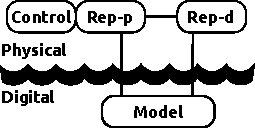
\includegraphics[width=300px]{mcrpd}}
	\caption{The MCRpd model of Ullmer \& Ishii for \acp{TUI}}
	\label{mcrpd}
\end{figure}

\acp{TUI} in general attempt to use the physical appearance of an object to communicate its virtual affordances \cite{Bellotti2002}. A user working with a \ac{GUI} only manipulates virtual objects, whereas \acp{TUI} allow the user to manipulate both physical and virtual objects, which coexist and share information with each other \cite{Shaer2004}. In a \ac{TUI}, the behaviour of a physical object is determined by the object's interactions with other physical and virtual objects - this is also the case in a smart environment.

Ullmer and Ishii \cite{Ullmer2000} extended the traditional \ac{MVC} model for \acp{TUI}, as shown in Figure \ref{mcrpd}. They distinguish between the physical and digital domains by placing the physical domain above the waterline, and the digital domain below the waterline. The model element is carried over from the \ac{MVC} model and represents the intangible digital information. The control element is also carried over from the \ac{MVC} model, while the view element is split into two subcomponents: 

\begin{itemize}
	\item Physical representations (Rep-p) -- represents the physically embodied elements of tangible interfaces
	\item Digital representations (Rep-d) -- represents the computationally mediated components of tangible interfaces without embodied form, for example video and audio, that can be observed in the physical world  
\end{itemize}

\marginpar{The interaction model introduced in Section \ref{InteractionModel} was inspired by the \ac{MCRpd} model.}

In a tangible interface, the physical representations (Rep-p) are computationally coupled to the underlying digital information (model), as well as perceptually coupled to the computationally mediated digital representations (Rep-d). 


	
	
\subsection{Foley's linguistic model}

	Foley's model defines the following levels \cite{DeRuiter1988}:
	
	\begin{itemize}
		\item Conceptual level - definition of main concepts and the possible commands (equivalent to user model \cite{Buxton1983})
		\item Semantic level - defines the meaning of the commands
		\item Syntactic level - describes the form of the command and parameters (syntax)
		\item Lexical level - defines lowest input symbols and their structure
	\end{itemize}
	
	Buxton \cite{Buxton1983} extended Foley's model to include a pragmatic level that defines the issues of gesture type (e.g. pointing with a tablet versus a mouse), device location and spatial placement. While a keystroke will be defined at lexical level, the homing time and pointing time will be defined at pragmatic level. Buxton had the foresight to comment on the difficulty of multi-device environments where the different levels are managed by different entities. He noted that it has a strong effect on the semantics of the interactions that could be supported: If the computing environment is managed by one entity, the semantics and functional capabilities by another, and the user interface by yet another, there is an inherent danger that the decisions of the one will adversely affect the other. 
	
	Dix et al \cite{Dix2008} noted that Buxton's work emphasised the way in which the lexical level design of the physical interface can simplify syntax in interaction. These ideas have been extended by Ullmer et al \cite{Ullmer2005} into a \emph{digital syntax} that is embodied by the physical design, resulting in a grammar for mapping physical relationships into digital representations.
	
	
\subsubsection{Arch/Slinky model}
	
	Bass et al \cite{Bass1992} contend that no single software architecture will satisfy all the design goals of an interactive system. With the Arch/Slinky model the buffering of a system from changes in technology was selected as the most important criterium. Here are some of the other design criteria they defined, which we consider to be especially important to ubiquitous computing systems:
	
	\begin{itemize}
		\item target system performance (e.g. size and speed)
		\item 	buffering from changes in application domain and hardware platform
		\item 	conceptual simplicity
		%\item 	complexity of specification
		\item 	target system extensibility
		\item 	compatibility with other systems
	\end{itemize}
	
	 They define an \emph{application} to be the total system that is developed for its end users, while the \emph{application domain} is the field of interest of, or reason for, the application. They also extended the definition of \ac{UIMS} to a  \ac{UIRS} - the run-time environment of an interactive application.
	
	The Arch model creates a bridge between the physical interaction device and the application domain. The following 5 components are defined:
	
	\begin{itemize}
		\item Interaction Toolkit Component - implements the physical interaction with the user (also called physical level)
		\item Presentation Component - provides a set of implementation-independent objects, e.g. a ``selector'' object can be implemented by both radio buttons or a drop-down menu in a GUI (also called lexical level)
		\item Dialogue Component - does task-level sequencing and maps between domain-specific and UI-specific formalisms (also called dialogue level)
		\item Domain Adaptor Component - triggers domain-initiated tasks, organises domain data, detects and reports semantic errors (also called functional core adapter)
		\item Domain-specific Component - controls, manipulates and retrieves domain data
	\end{itemize}

The separation of functionality into the different components was done to minimise the effects of changes in technology. The Slinky meta-model is a generalisation of the Arch model, providing a set of Arch models with different weights assigned to each component.

\subsubsection{Nielsen's virtual protocol model}
\label{nielsenVPM}
Nielsen's virtual protocol model for human-computer interaction \cite{Nielsen1986} was inspired by the 7-layer OSI model for computer networks, as shown in Table \ref{VirtualProtocolModel}. The task layer deals with general computer-related concepts that are representations of the real world concepts from level 7, that may have to be realised by a sequence of operations from level 5. Level 5 handles the meaning of the interaction, where there are a finite number of concepts in the system and each have an exact definition. The lexical tokens on level 4 (``DELETE 27'') realises the semantic command ``remove a specific line''. Lexemes are information-carrying units that do not have any meaning by themselves. Screen layout could be considered a two-dimensional syntax that can also be defined in terms of lexical tokens. Direct manipulation \cite{Shneiderman1997} could be seen as using the syntax level to mirror the semantic level.

Nielsen compared his model to Foley's model and Buxton's extended version, as well as an earlier model by Moran called \ac{CLG} that consisted of six levels: task level, semantic level, syntactic level, interaction level and device level \cite{Nielsen1986}. He noticed that all models seem to agree on the visible (defining the form) part of the communication, as well as the invisible part (defining the meaning). Nielsen noted that Foley's model does not include the real-world concepts of his goal level, or the hardware-related detail of his physical level.

According to Nielsen the purpose of his model is to improve the usability of software. He noted that some people will consider it a useful abstraction, while others will prefer other models, similar to how everybody has their own favourite programming language.


\begin{table}
    \myfloatalign
  \begin{tabularx}{\textwidth}{Xll} 
	\toprule
    \tableheadline{Level} & \tableheadline{Layer} & \tableheadline{Example} \\ 
    \midrule

	7 & Goal & Want to delete the last section of a document\\
	6 & Task & Delete the last six lines of the edited text\\
	5 & Semantic & Remove a line with a given line number\\
	4 & Syntax & DELETE 27 \\
	3 & Lexical & DELETE, DEL or other lexical token \\
	2 & Alphabetic & Letter ``D'' or other lexeme \\
	1 & Physical & User presses D-key on keyboard \\
	
    \bottomrule
  \end{tabularx}
  \caption{Nielsen's virtual protocol model}
  \label{VirtualProtocolModel}
\end{table}



\subsubsection{The ASUR interaction model}
\label{theasurinteractionmodel}

\ac{ASUR} is a notation-based model to describe user-system interaction in mixed interactive systems \cite{Dubois2008} at design-time. It describes the physical and digital entities that make up a mixed system and uses directed relationships (arrowed lines) to express physical and/or digital information flows and associations between the components.

Both components and relationships may have characteristics. For components, this includes the location where the information is perceived (e.g. top of table) and action/sense required from the user (e.g. sight, touch or physical action). For relationships, characteristics include the dimensionality of the information (e.g. 2D or 3D) and the type of language used (e.g. text or graphics).

A sequence of such entities and their relationships in an interaction forms an \emph{interaction path}. The interaction exchange or action between elements in the path is conducted via one or more \emph{interaction channels} along which information or action is communicated. An interaction channel may be described in terms of its properties, either physical or digital depending on the channel, e.g. a digital channel may be described in terms of bandwidth, uptime and the nature of the connection. Adaptors are used transform information from the physical environment to the digital world and vice versa. An accelerometer for example may be modelled as a separate device, but if integrated into smart phones it can be abstracted away as part of an interaction path. 

Interaction carriers are mediating entities that are necessary for information communication. Passive carriers can carry and store part of the information communicated along an interaction path, e.g. a tangible object left in a particular position. Active carriers are transmitters of non-persistent information along the interaction path, e.g. a stylus used to transmit a precise position on a touch screen. Contextual entities are physical entities involved in an interaction (e.g. a table), and are also considered mediating entities.

The intended user model refers to what the user should know about the interaction in order to carry it out successfully. It may refer to one atomic interaction path (e.g. a channel, source and destination), or it may refer to more complex paths. 

An interaction group refers to a set of entities and channels that together have properties that are relevant to a particular design issue. Some of these groups will be applicable to any design, while others will depend on the task and context:

\begin{itemize}
\item Entities and channels may be \emph{grouped for feedback}, to identify an interaction flow that links the response of the system to the actions of the user.

\item User interface elements may be linked to application concepts in order to express a semantic association. The goal is to help the user to cognitively unify elements of the group (helping to establish the intended user model).

\item Sets of input (e.g. speech input for gesture input - ``put that there'') that must be combined to perform a certain task, may be grouped for multimodal interaction.

\item A grouping may be used to assert that a set of services must reside on the same machine or be distributed over multiple devices.

\item A grouping of paths may show information flows among or between multiple users.

\end{itemize}

An advantage of the \ac{ASUR} interaction model is that it combines both the physical and digital dimensions of user-system interaction.

% Dubois and Gray \cite{Dubois2008} consider their interaction model similar to that of Coutrix et al \cite{Coutrix2006} (described in section \ref{mixedreality}), in the sense that both combine the physical and digital dimensions of the interaction. 
% 
% \subsubsection{The Mixed Reality interaction model}
% \label{mixedreality}
% 
% An interaction model aims at providing a framework for guiding designers to create interactive systems \cite{Coutrix2006}, characterised by their:
% 
% \begin{itemize}
% \item descriptive/classification power: describes existing interfaces and classifies them
% 
% \item generative power: helps designers create new designs
% 
% \item comparative power: helps to assess multiple design alternatives
% 
% \end{itemize}
% 
% Given that \emph{d} is a physical device that acquires or delivers information, and \emph{l} is an interaction language that defines a set of well-formed expressions that convey meaning, a modality \emph{m} is a pair \emph{(d,l)}. Modalities that define the link between digital and physical properties are known as \emph{linking modalities}, and modalities used by the user to interact with the mixed environment are known as \emph{interaction modalities}.
% 
% \begin{itemize}
% \item An input linking modality ($d_o^i, l_o^i$) is responsible for
% 
% \begin{enumerate}
% \item acquiring a subset of \emph{physical properties}, using a $d_o^i$ device (object input device)
% 
% \item interpreting these \emph{acquired physical data} in terms of \emph{digital properties}, using a language $l_o^i$ (object input language)
% 
% \end{enumerate}
% 
% \item An output linking modality is in charge of
% 
% \begin{enumerate}
% \item generating data based on the set of \emph{digital properties}, using a language $l_o^o$ (object output language),
% 
% \item translating these \emph{generated physical data} into perceivable \emph{physical properties} thanks to a device $d_o^o$ (object output device).
% 
% \end{enumerate}
% 
% \end{itemize}
% 
% An interaction language $l_i^i$ translates the digital properties of a mixed tool into elementary task to be performed (e.g. collect select puzzle piece). Using the linking modalities, different modalities may be generated to describe the mixed tool.

	
\section{Task models}
\label{interactionTasks}
	
	Foley \cite{Foley1984} describes a taxonomy of input devices that are structured according the graphic subtasks they can perform: position, orientation, select, path, quantify and text entry. He defined these subtasks as six basic interaction tasks (BITs) that correspond to the lexical level. A BIT is the smallest unit of information entered by a user that is meaningful in the context of the application. He noted that there are far too many interaction techniques to give an exhaustive list, and that it is impossible to to anticipate which new techniques may be created. In table \ref{InteractionTasks} we map them to possible logical and physical interaction devices. The six types of logical devices were also defined by Foley in \cite{Foley1996}.
	
	
	\begin{table}
	    \myfloatalign
	  \begin{tabularx}{\textwidth}{Xll} 
		\toprule
	    \tableheadline{Interaction Task} & \tableheadline{Logical Device} & \tableheadline{Physical Device} \\ 
	    \toprule

		Position & Locator & Tablet \\
		\cline{1-2}

		\multirow{2}{*}{Select} & Choice & Touch Panel\\
		 						& Pick & Trackball/Mouse\\
		\cline{1-2}						
		Path & Stroke & Joystick \\
		\midrule
		Quantify & Valuator & Dials\\
		\midrule
		Text entry & String & Keyboard  \\
		\midrule
		Orient & & \\

	    \bottomrule
	  \end{tabularx}
	  \caption{Interaction tasks mapped to logical and physical interaction devices}
	\label{InteractionTasks}
\end{table}
	

	
	Some characteristics of the physical interaction devices are not shown in the table.  The positioning of tablets and touch panels are \emph{absolute}, while that of trackballs, joysticks and mice are \emph{relative}. A touch panel is considered \textit{direct}, as the user directly points at the screen, while a tablet is \textit{indirect}. Joysticks, tablets and mice are \emph{continuous}, while a keyboard is \emph{discrete}. Dials can either be \emph{bounded} or \emph{unbounded}.
	
	The \emph{positioning} interaction task involves specifying an (x,y) or (x,y,z) position. Characteristics of this task include different coordinate systems, resolution and spatial feedback. The \emph{select} interaction task involves choosing an element from a choice set, while the \emph{text} interaction task entails entering character strings to which the system does not assign specific meaning. The \emph{quantify} interaction task involves specifying a numeric value between some minimum and maximum value. The \emph{path} interaction task consists of specifying a number of positions over a specific time or distance interval. The \emph{orient} interaction task is also called \emph{rotate}, but is not often used \cite{DeRuiter1988}.
	
	Card et al \cite{Card1991} argued that the Foley taxonomy has not tried to define a notion of completeness, and is thus not generic enough. They pointed out that single devices appear many times in the levels of the tree, which makes it difficult to understand the similarities among devices. MacKinlay, Card and Robertson \cite{MacKinlay1990} extended Buxton's work to propose additional physical properties that underly most devices. They follow mappings from the raw physical transducers of an input device into the semantics of the application.
	
	Dix et al \cite{Dix2008} noted that Card et al's analysis is not only relevant to GUIs, as they used a running example of a radio with knobs and dials. Their work not only abstracts devices into classes, but also takes into account that rotating a dial is different from moving a slider, i.e. the physical nature of the interaction is also important.
	
	
	 Ballagas et al \cite{Ballagas2006} surveyed interaction techniques that use mobile phones as input devices to ubiquitous computing environments, and used Foley's six interaction tasks as a framework for their analysis. In their work on iStuff \cite{Ballagas2003} they state that the set of interactions tasks are only sufficient for describing graphical user interfaces, not physical user interfaces, or user interfaces in general. The same paper notes that Buxton's taxonomy, and the extension by MacKinlay, Card and Robertson, is too narrow for ubiquitous computing environments, as it does not classify devices with different modalities and only describes input devices. They extended the taxonomy further to describe attributes like direction and modality. The direction attribute is used to indicate whether a device provides input, output or both. The modality attribute describes different visual, auditory haptic and manual modalities for input and output. Additional attributes they identified include directionality/scope (where a device is targeted to one, many, or all the users in a room) and mount time (the effort necessary to use an interaction device).
	
	
\subsection{Another approach to task modelling: ANSI/CEA-1028}
\label{cea2018}

	A task model is often defined as a description of an interactive task to be performed by the user of an application through the application's user interface. Individual elements in a task model represent specific actions that the user may undertake. Information on subtask ordering as well as conditions on task execution is also included in the model~\cite{Limbourg2004}. In traditional user interface design, task models are used only at design time and then discarded \cite{Rich2009}. A task-based user interface uses a task model at runtime to guide the user.

	A task is commonly defined as an activity performed to reach a certain goal. A goal of a task is considered to be a specific state that is reached after the successful execution of a task. Tasks vary widely in their time extent. Some occur over minutes or hours (like listening to a song or watching a TV show), while others are effectively instantaneous, like switching on the TV.

	ANSI/CEA-1028 \cite{Rich2009} uses a single uniform task representation, compared to other representations where high-level tasks (goals) are separated from low-level tasks (actions). It does so at all levels of abstraction, providing more flexibility when adjusting the level of granularity. %We consider this a worthwhile option to explore as this allows for the simplification of the model.

	In \cite{VanWelie1998} it is suggested that task models should be based on an ontology that describes the relevant concepts and the relationships between them, independently of any used graphical representations. This also allows for different visualisations of the same task model. Task decomposition is the most common ingredient of task models. This creates a task tree or hierarchy that can easily be modelled by an ontology. The most important purpose of a task is that it changes something, otherwise it has no reason for existing.

\marginpar{Van Welie et al \cite{VanWelie1998} state that task models should be able to represent the psychological, social, environmental and situational aspects of agents and their tasks. This is why we consider runtime task models a good fit for the \ac{BDI} model used for constructing intelligent agents.}
	
	

\section{Semantic models}
%\input{interactionFrogger}
\label{interactionFrogger}
The Frogger framework, as was introduced by Wensveen \cite{Wensveen2005}, describes user interaction in terms of the information a user perceives (like feedback and feedforward), and the nature of this information. It distinguishes between inherent, augmented and functional information. These types of information can serve as couplings between user actions and the systems' functions in time, location, direction, modality, dynamics and expression. Although the framework was designed to describe the interaction with electronic devices and their interfaces, many of the concepts in the framework are applicable to interactions with systems of devices as well.

When a user performs an action and the device responds with information that is directly related to the function of that product (lighting switching on when a light switch is operated), we speak of \emph{functional feedback}. When a device has more than one functionality, functional feedback should be viewed with respect to the users' intentions and goals when performing the action. If there is no direct link between a user's action and the direct function of the product, or when there is a delay, \emph{augmented feedback} (also known as indicators \cite{Thimbleby2007}) can be considered to confirm a user's action. This feedback is usually presented in the form of lights, sounds or labels. \emph{Inherent feedback} is directly coupled (inherently) to the action itself, like the feeling of displacement, or the sound of a button that is pressed.

While feedback is information that occurs after or during the interaction, feedforward is the information provided to the user before any action has taken place. \emph{Inherent feedforward} communicates what kind of action is possible, and how one is able to carry out this action. Inherent feedforward is in many ways similar to the concept of affordances\marginpar{Affordances were discussed in Section \ref{Affordances}. }, revealing the action possibilities of the product or its controls \cite{Wensveen2005}. When an additional source of information communicates what kind of action is possible it is considered \emph{augmented feedforward}.  
\emph{Functional feedforward} communicates the more general purpose of a product. This type of information often relies on association, metaphors and the sign function of products, which are described by theories such as product semantics \cite{Krippendorff2006}. Good practice in creating inherent feedforward is making the functional parts of a product visible, informing users about the functionality of the product \cite{Norman1998}.	

%\footnote{Affordance is a term coined by Gibson in 1979 and introduced to the design community by Norman \cite{Norman1998}. It is the property of an object that appeals to our sensory-motor skills, like a door handle ``affords'' to be grabbed and a chair ``affords'' to be sat on.}
	
\subsection{Models of intentionality}
\label{intentionalSpectrum}
	
	At the semantic level, we are interested in the meaning of the action. A gesture may mean nothing, until it encounters for instance a light switch \cite{Bongers2007}. In traditional software applications, a user is expected to have a clear intention of what he/she wants to achieve, with purposeful and direct actions. In ubiquitous computing scenarios, the interactions are less explicit. Input is implicit, sensor-based and ``calm'', and output is ambient and non-intrusive. With \emph{incidental interactions} \cite{Dix2004}, a user performs an action for some purpose (say opening a door to enter a room), the system senses this and incidentally uses it for some purpose of which the user is unaware (e.g. adjust the room temperature), affecting the user's future interaction with the system.
	
\begin{figure}
	\centering
	\centerline{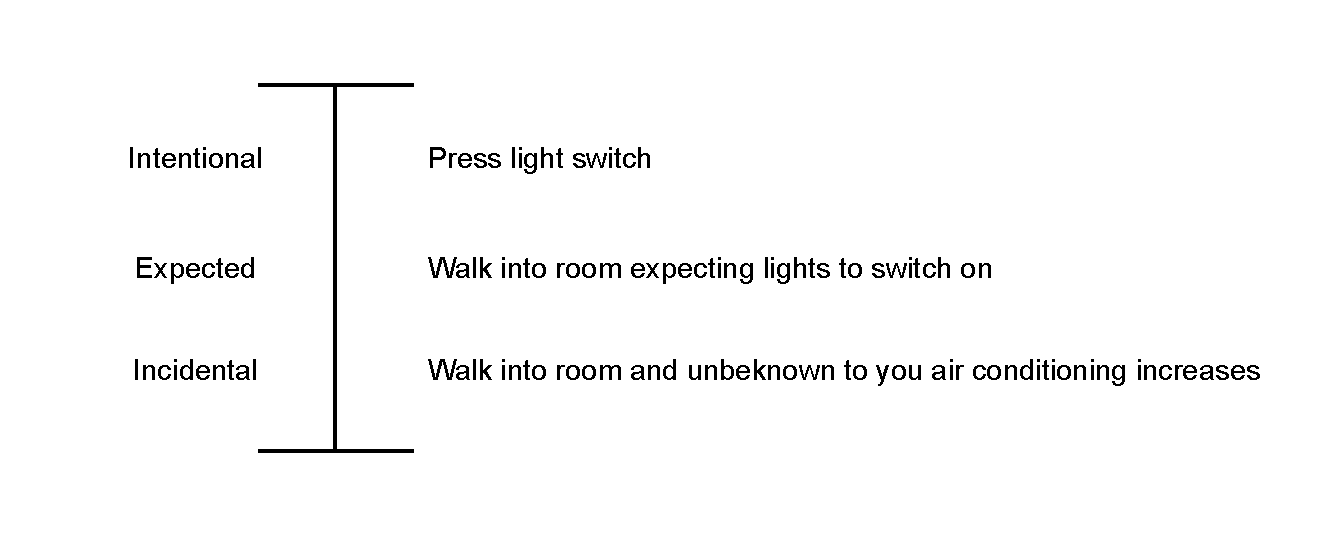
\includegraphics[width=300px]{continuum}}
	\caption{The continuum of intentionality}
	\label{continuum}
\end{figure}	

	The \emph{continuum of intentionality} in Figure \ref{continuum} has normal, intentional interactions at the one end of the spectrum (e.g. pressing a light switch), expected interactions in the middle (e.g. walking into a room expecting the lights to go on), and incidental interactions at the other end. As users become more aware of the interactions happening around them, they move through the continuum toward more purposeful interaction. For example, with \emph{comprehension} an incidental interaction (lights turning on when you enter the car) turns into an expected interaction. With \emph{co-option}, an expected interaction turns into an intended interaction (e.g. deliberately opening and closing the car door to turn on the light).

	Incidental interactions do not fit existing interaction models based on the conventional intentional cycle, like Norman's Action Cycle Diagram \cite{Norman1998}. The purpose of the user's activity is distinct to the intended outcomes of the system. Feedback may be unobtrusive (and not noticed), or delayed (like the temperature slowly changing). There are two tasks that are occurring:

	\begin{itemize}
	\item The user's purposeful activity
	\item The task that the incidental interaction is attempting to support/achieve
	\end{itemize}

We try to improve this comprehension by actively involving users in configuring the relationships between the smart objects in their environment. When users are able to explore and manipulate the relationships between the smart objects, it becomes easier for them to begin to comprehend how things work (or can potentially work together). They can project their experiences with a part of a smart environment to see what may potentially work for other parts of the environment as well. %we can close this loop in the discussion with results from the user experiment.
By allowing users to configure their smart environment themselves, they are in control of deciding how the environment responds to their actions.

%end TiiS

\section{Outlook}

We build further on many of the concepts and proposals reviewed in this chapter. In particular, we focus on configuring the connections between the devices in Chapters \ref{DesignIteration1} to \ref{DesignIteration3} and Chapter \ref{SemanticConnectionsTheory}, while serendipitous interoperability and sharing information between devices form the cornerstones of Chapter \ref{DeviceCapabilityModelling} and Chapter \ref{EventModelling}. 